\begin{figure}
   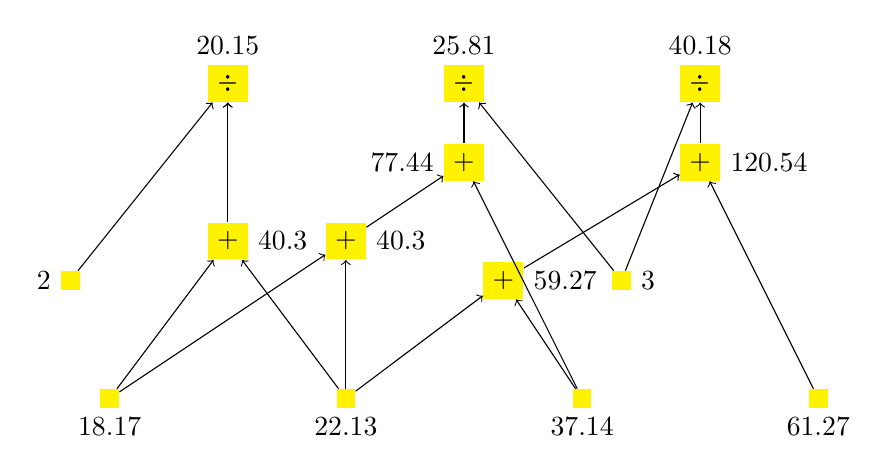
\begin{tikzpicture}
      \begin{scope}[name prefix = input-]
         \node[fill=yellow, label={below:{18.17}}] (1) at (0, 0) {};
         \node[fill=yellow, label={below:{22.13}}] (2) at  (3, 0) {};
         \node[fill=yellow, label={below:{37.14}}] (3) at  (6, 0) {};
         \node[fill=yellow, label={below:{61.27}}] (4) at (9, 0) {};
      \end{scope}
      
      \begin{scope}[name prefix = len-]
         \node[fill=yellow, label=left:2] (div2) at (-0.5, 1.5) {};
         \node[fill=yellow, label=right:3] (div3) at (6.5, 1.5) {};
      \end{scope}

      \begin{scope}[name prefix = add-]
         \node[fill=yellow, label={[label position = 0] $40.3$}] (1) at (1.5, 2) {+};
         \node[fill=yellow, label={[label position = 0] $40.3$}] (2) at (3, 2) {+};
         \node[fill=yellow, label={[label position = 180] $77.44$}] (3) at (4.5, 3) {+};
         \node[fill=yellow, label={[label position = 0] $59.27$}] (4) at (5, 1.5) {+};
         \node[fill=yellow, label={[label position = 0]$120.54$}] (5) at (7.5, 3) {+};
      \end{scope}

      \begin{scope}[name prefix = div-]
         \node[fill=yellow, label={$20.15$}] (1) at (1.5, 4) {÷};
         \node[fill=yellow, label={$25.81$}] (2) at (4.5, 4) {÷};
         \node[fill=yellow, label={$40.18$}] (3) at (7.5, 4) {÷};
      \end{scope}
      
      \begin{scope}
         \draw[->] (input-1) -- (add-1);
         \draw[->] (input-2) -- (add-1);
         \draw[->] (add-1) -- (div-1);
         \draw[->] (len-div2) -- (div-1);
         \draw[->] (add-1) -- (div-1);
         \draw[->] (input-1) -- (add-2);
         \draw[->] (input-2) -- (add-2);
         \draw[->] (add-2) -- (add-3);
         \draw[->] (input-3) -- (add-3);
         \draw[->] (add-3) -- (div-2);
         \draw[->] (len-div3) -- (div-2);
         \draw[->] (input-2) -- (add-4);
         \draw[->] (input-3) -- (add-4);
         \draw[->] (input-4) -- (add-5);
         \draw[->] (add-4) -- (add-5);
         \draw[->] (add-5) -- (div-3);
         \draw[->] (len-div3) -- (div-3);
      \end{scope}
   \end{tikzpicture}
   \caption{Portion of the dependence graph computed for the moving averages example.}
   \label{fig:core:mavg}
\end{figure}